\chapter{Compound Angles}
Algebraic sum of two or more angles is called a {\it compound angle}. If $A, B, C$ are any angle then $A + B, A - B, A -
B + C, A + B + C, A - B - C, A + B -C$ etc. are all compound angles.

\section{The Addition Formula}
$$\sin(A + B) = \sin A\cos B + \sin B\cos A$$
$$\cos(A + B) = \cos A\cos B - \sin A\sin B$$
$$\tan(A + B) = \frac{\tan A + \tan B}{1 - \tan A\tan B}$$

\begin{center}
  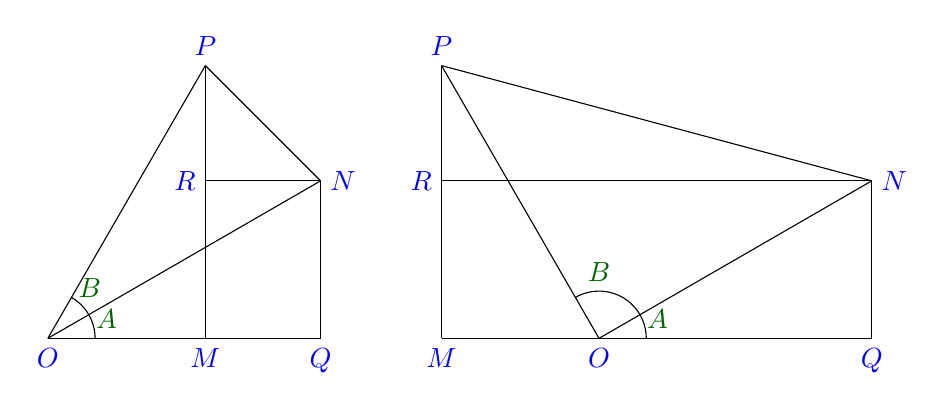
\begin{tikzpicture}
    \draw (0, 0) -- (3.464, 0);
    \draw (3.464, 0) -- (3.464, 2);
    \draw (0, 0) -- (3.464, 2);
    \draw (0, 0) -- (2, 0);
    \draw (2, 0) -- (2, 3.464);
    \draw (0, 0) -- (2, 3.464);
    \draw (2, 3.464) -- (3.464, 2);
    \draw (3.464, 2) -- (2, 2);
    \draw (.6, 0) arc[start angle=0, end angle=30, radius=0.6];
    \draw (.52, .3) arc[start angle=30, end angle=60, radius=0.6];
    \draw [blue] (0, 0) node[anchor=north] {$O$};
    \draw [blue] (2, 0) node[anchor=north] {$M$};
    \draw [blue] (3.464, 0) node[anchor=north] {$Q$};
    \draw [blue] (3.464, 2) node[anchor=west] {$N$};
    \draw [blue] (2, 2) node[anchor=east] {$R$};
    \draw [blue] (2, 3.464) node[anchor=south] {$P$};
    \draw [black!60!green] (1, 0) node[anchor=south east] {$A$};
    \draw [black!60!green] (.8, .4) node[anchor=south east] {$B$};

    \draw (7, 0) -- (10.464, 0);
    \draw (10.464, 0) -- (10.464, 2);
    \draw (7, 0) -- (10.464, 2);
    \draw (7, 0) -- (5, 0);
    \draw (5, 0) -- (5, 3.464);
    \draw (7, 0) -- (5, 3.464);
    \draw (10.464, 2) -- (5, 3.464);
    \draw (10.464, 2) -- (5, 2);
    \draw (7.6, 0) arc[start angle=0, end angle=30, radius=0.6];
    \draw (7.52, .3) arc[start angle=30, end angle=120, radius=0.6];
    \draw [blue] (7, 0) node[anchor=north] {$O$};
    \draw [blue] (5, 0) node[anchor=north] {$M$};
    \draw [blue] (10.464, 0) node[anchor=north] {$Q$};
    \draw [blue] (10.464, 2) node[anchor=west] {$N$};
    \draw [blue] (5, 2) node[anchor=east] {$R$};
    \draw [blue] (5, 3.464) node[anchor=south] {$P$};
    \draw [black!60!green] (8, 0) node[anchor=south east] {$A$};
    \draw [black!60!green] (7, .6) node[anchor=south] {$B$};
  \end{tikzpicture}
\end{center}

Consider the diagram above. $PM$ and $PN$ are perpendicualr to $OQ$ and $ON$. $RN$ is parallel to
$OQ$ and $NQ$ is perpendicular to $OQ$. The left diagram represents the case when sum of angles is an acute angle
while the right diagram represents the case when sum of angles is an obtuse angle.

$\angle RPN = 90^{\circ} - \angle PNR = \angle RNO = \angle NOQ = \angle A$

Now we can write, $\sin(A + B) = \sin QOP = \frac{MP}{OP} = \frac{MR + RP}{OP} = \frac{QN}{OP} + \frac{RP}{OP}$

$=\frac{QN}{ON}\frac{ON}{OP} + \frac{RP}{NP}\frac{NP}{OP} = \sin A\cos B + \cos A\sin B$

Also, $\cos(A + B) = \cos QOP = \frac{OM}{OP} = \frac{OQ - MQ}{OP} = \frac{OQ}{ON}\frac{ON}{OP} - \frac{RN}{NP}\frac{NP}{OP}$

$= \cos A\cos B - \sin A\sin B$

These two results lead to $\tan (A + B) = \frac{\tan A + \tan B}{1 - \tan A\tan B}$

We have shown that addition formula is true when angles involved are acute angles. The same proof can be applied to prove the
results for all values of $A$ and $B$.

Consider $A' = 90^{\circ} + A \therefore \sin A' = \cos A$ and $\cos A' = \sin A$

$\sin(A' + B) = \cos (A + B) = \cos A\cos B - \sin A\sin B = \sin A'\cos B + \cos A'\sin B$

Similarly $\cos(A' + B) = -\sin(A + B) = -\sin A\cos B - \sin B\cos A = \cos A'\cos B - \sin A'\sin B$

We can prove it again for $B' = 90^{\circ} + B$ and so on by increasing the values of $A$ and $B$. Then we can
again increase values by $90^{\circ}$ and proceeding this way we see that the formula holds true for all values of $A$
and $B$.

\section{The Subtraction Formula}
$$\sin(A - B) = \sin A\cos B - \sin B\cos A$$
$$\cos(A - B) = \cos A\cos B + \sin A\sin B$$
$$\tan(A - B) = \frac{\tan A - \tan B}{1 + \tan A\tan B}$$

\begin{center}
  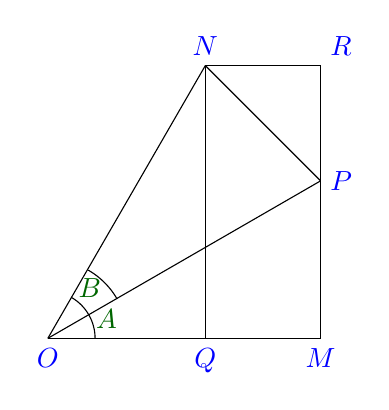
\begin{tikzpicture}
    \draw (0, 0) -- (3.464, 0);
    \draw (3.464, 0) -- (3.464, 2);
    \draw (0, 0) -- (3.464, 2);
    \draw (0, 0) -- (2, 0);
    \draw (2, 0) -- (2, 3.464);
    \draw (0, 0) -- (2, 3.464);
    \draw (2, 3.464) -- (3.464, 2);
    \draw (2, 3.464) -- (3.464, 3.464);
    \draw (3.464, 3.464) -- (3.464, 2);
    \draw (.6, 0) arc[start angle=0, end angle=60, radius=0.6];
    \draw (.88, .5) arc[start angle=30, end angle=60, radius=1];
    \draw [blue] (0, 0) node[anchor=north] {$O$};
    \draw [blue] (2, 0) node[anchor=north] {$Q$};
    \draw [blue] (3.464, 0) node[anchor=north] {$M$};
    \draw [blue] (3.464, 2) node[anchor=west] {$P$};
    \draw [blue] (3.464,3.464) node[anchor=south west] {$R$};
    \draw [blue] (2, 3.464) node[anchor=south] {$N$};
    \draw [black!60!green] (1, 0) node[anchor=south east] {$A$};
    \draw [black!60!green] (.8, .4) node[anchor=south east] {$B$};
  \end{tikzpicture}
\end{center}

Conside the diagram above. The angle $MOP$ is $A - B.$ We take a point $P,$ and draw $PM$ and $PN$
perpendicular to $OM$ and $ON$ respectively. From $N$ we draw $NQ$ and $NR$ perpendicular to
$OQ$ and $MP$ respectively.

$\angle RPN = 90^{\circ} - \angle PNR = \angle QON = A$

Thus, we can write $\sin(A - B) = \sin MOP = \frac{MP}{OP} = \frac{MR - PR}{OP} = \frac{QN}{ON}\frac{ON}{OP} -
\frac{PR}{PN}\frac{PN}{OP}$

Thus, $\sin(A - B) = \sin A\cos B - \cos A\sin B$

Also, $\cos(A - B) = \frac{OM}{OP} = \frac{OQ + QM}{OP} = \frac{OQ}{ON}\frac{ON}{OP} + \frac{RN}{NP}\frac{NP}{OP}$

$= \cos A\cos B + \sin A\sin B$

We have shown that subtraction formula is true when angles involved are acute angles. The same proof can be applied to prove the
results for all values of $A$ and $B$.

From the results obtained we find upon division that $\tan(A - B) = \frac{\tan A - \tan B}{1 + \tan A\tan B}$

\section{Important Deductions}
\begin{enumerate}
\item $\sin(A + B)\sin(A - B) = \sin^2A - \sin^2B = \cos^2B - \cos^2A$

$\text{L.H.S.}= (\sin A\cos B + \sin B\cos A)(\sin A\cos B - \sin B\cos A)$

  $= \sin^2A\cos^2B - \sin^2B\cos^2A = \sin^2A(1 - \sin^2B) - \sin^2B(1 - \sin^2A)$

  $= \sin^2A - \sin^2A\sin^2B - \sin^2B + \sin^2B\sin^2A$

  $=\sin^2A - \sin^2B = (1 - \cos^2A) - (1 - \cos^2B)$

  $= \cos^2B - \cos^2A$

\item $\cos(A + B)\cos(A - B) = \cos^2A - \sin^2B = \cos^2B - \sin^2A$

$\text{L.H.S.} =(\cos A\cos B - \sin A\sin B)(\cos A\cos B + \sin A\sin B)$

  $= \cos^2A\cos^2B - \sin^2A\sin^2B$

  $= \cos^2A(1- \sin^2B) - (1 - \cos^2A)\sin^2B$

  $=\cos^2A - \cos^2A\sin^2B - \sin^2B + \cos^2A\sin^2B$

  $= \cos^2A - \sin^2B = \cos^2B - \sin^2A$

\item $\cot(A + B) = \frac{\cot A\cot B - 1}{\cot B + \cot A}$

  $\text{L.H.S.} = \cot(A + B) = \frac{\cos(A + B)}{\sin(A + B)}$

  $= \frac{\cos A\cos B - \sin A\sin B}{\sin A\cos B + \cos A\sin B}$

  Dividing numerator and denominator by $\sin A\sin B$

  $= \frac{\cot A\cot B - 1}{\cot B + \cot A}$

\item $\cot(A - B) = \frac{\cot A\cot B + 1}{\cot B - \cot A}$

  L.H.S. $= \cot(A - B) = \frac{\cos(A - B)}{\sin(A - B)}$

  $= \frac{\cos A\cos B + \sin A\sin B}{\sin A\cos B - \cos A\sin B}$

  Dividing numerator and denominator by $\sin A\sin B$

  $= \frac{\cot A\cot B + 1}{\cot B - \cot A}$

\item $\tan(A + B + C) = \frac{\tan A + \tan B + \tan C - \tan A\tan B\tan C}{1 - \tan A\tan B - \tan B\tan C - \tan C\tan A}$

   L.H.S. $= \tan[(A + B) + C] = \frac{\tan(A + B) + \tan C}{1 - \tan(A + B)\tan C}$

   $= \frac{\frac{\tan A + \tan B}{1 - \tan A\tan B} + \tan C}{1 - \frac{\tan A + \tan B}{1 - \tan A\tan B}\tan C}$

   $= \frac{\frac{\tan A + \tan B + \tan C - \tan A\tan B\tan C}{1 - \tan A\tan B}}{\frac{1 - \tan A\tan B - \tan B\tan C -
   \tan C\tan A}{1 - \tan A\tan B}}$

   $= \frac{\tan A + \tan B + \tan C - \tan A\tan B\tan C}{1 - \tan A\tan B - \tan B\tan C - \tan C\tan A}$
\end{enumerate}

\section{To express $a\cos\theta + b\sin\theta$ in the form of $k\cos\phi$ or $k\sin\phi$}
$a\cos\theta + b\sin\theta = \sqrt{a^2 + b^2}\left(\frac{a}{\sqrt{a^2 + b^2}}\cos\theta + \frac{b}{\sqrt{a^2 +
b^2}}\sin\theta\right)$

Let $\cos\alpha = \frac{a}{\sqrt{a^2 + b^2}}$ then $\sin\alpha = \frac{b}{\sqrt{a^2 + b^2}}$

Thus, $a\cos\theta + b\sin\theta = \sqrt{a^2 + b^2}(\cos\alpha\cos\theta + \sin\alpha\sin\theta)$

$= \sqrt{a^2 + b^2}\cos(\theta - \alpha) = k\cos\phi$ where $k = \sqrt{a^2 + b^2}$ and $\phi = \theta - \alpha$

Alternatively, if $\frac{a}{\sqrt{a^2 + b^2}} = \sin\alpha$ then $\frac{b}{\sqrt{a^2 + b^2}} = \cos\alpha$

Thus, $a\cos\theta + b\sin\theta = \sqrt{a^2 + b^2}(\sin\alpha\cos\theta + \cos\alpha + \sin\theta)$

$= \sqrt{a^2 + b^2}\sin(\theta + \alpha) = k\sin\phi$ where $k = \sqrt{a^2+b^2}$ and $\phi = \theta + \alpha$

\section{Problems}
\begin{enumerate}
\item If $\sin\alpha = \frac{3}{5}$ and $\cos\beta = \frac{9}{41},$ find the values of $\sin(\alpha - \beta)$ and
   $\cos(\alpha + \beta)$.

\item If $\sin\alpha = \frac{45}{53}$ and $\sin\beta = \frac{33}{65},$ find the values of $\sin(\alpha - \beta)$ and
   $\sin(\alpha + \beta)$.

\item If $\sin\alpha = \frac{15}{17}$ and $\cos\beta = \frac{12}{13},$ find the values of $\sin(\alpha + \beta),
   \cos(\alpha - \beta)$ and $\tan(\alpha + beta)$.
\end{enumerate}

Prove the following:

\begin{enumerate}
\item $\cos(45^{\circ} - A)\cos(45^{\circ} - B) - \sin(45^{\circ} - A)\sin(45^{\circ} - B) = \sin(A + B)$.

\item $\sin(45^{\circ} + A)\cos(45^\circ - B) + \cos(45^{\circ} + A)\sin(45^\circ - B) = \cos(A - B)$.

\item $\frac{\sin(A - B)}{\cos A\cos B} + \frac{\sin(B - C)}{\cos B\cos C} + \frac{\sin(C - A)}{\cos C\cos A} = 0$.

\item $\sin 105^\circ + \cos 105^\circ = \cos 45^\circ$.

\item $\sin 75^\circ - \sin 15^\circ = \cos 105^\circ + \cos 15^\circ$.

\item $\cos\alpha\cos(\gamma - \alpha) - \sin\alpha\sin(\gamma - \alpha) = \cos\gamma$.

\item $\cos(\alpha + \beta)\cos\gamma - \cos(\beta + \gamma)\cos\alpha = \sin\beta\sin(\gamma - \alpha)$.

\item $\sin(n + 1)A\sin(n - 1)A + \cos(n + 1)A\cos(n - 1)A = \cos 2A$.

\item $\sin(n + 1)A\sin(n + 2)A + \cos(n + 1)A\cos(n + 2)A = \cos A$.

\item Find the value of $\cos 15^\circ$ and $\sin 105^\circ$.

\item Find the value of $\tan 105^\circ$.

\item Find the value of $\frac{\tan 495^\circ}{\cot 855^\circ}$.

\item Evaluate $\sin\left(n\pi + (-1)^n \frac{\pi}{4}\right),$ where $n$ is an integer.
\end{enumerate}

Prove the following:

\begin{enumerate}[resume]
\item $\sin 15^\circ = \frac{\sqrt{3} - 1}{2\sqrt{2}}$.

\item $\cos 75^\circ = \frac{\sqrt{3} - 1}{2\sqrt{2}}$.

\item $\tan 75^\circ = 2 + \sqrt{3}$.

\item $\tan 15^\circ = 2 - \sqrt{3}$.
\end{enumerate}

Find the value of following:

\begin{enumerate}[resume]
\item $\cos 1395^\circ$.

\item $\tan(-330^\circ)$.

\item $\sin 300^\circ {\rm cosec} 1050^\circ - \tan(-120^\circ)$.

\item $\tan\left(\frac{11\pi}{12}\right)$.

\item $\tan \left((-1)^n\frac{\pi}{4}\right)$.
\end{enumerate}

Prove the following:

\begin{enumerate}[resume]
\item $\cos 18^\circ - \sin 18^\circ = \sqrt{2}\sin 27^\circ$.

\item $\tan 70^\circ = 2\tan 50^\circ + \tan 20^\circ$.

\item $\cot\left(\frac{\pi}{4} + x\right)\cot\left(\frac{\pi}{4} - x\right) = 1$.

\item $\cos(m + n)\theta.\cos(m - n)\theta - \sin(m + n)\theta\sin(m - n)\theta = \cos 2m\theta$.

\item $\frac{\tan(\theta + \phi) + \tan(\theta - \phi)}{1 - \tan(\theta + \phi)\tan(\theta - \phi)} = \tan 2\theta$.

\item $\cos 9^\circ + \sin 9^\circ = \sqrt{2}\sin 54^\circ$.

\item $\frac{\cos 20^\circ - \sin 20^\circ}{\cos 20^\circ + \sin 20^\circ} = \tan 25^\circ$.

\item $\frac{\tan A + \tan B}{\tan A - \tan B} = \frac{\sin(A + B)}{\sin(A - B)}$.

\item $\frac{1}{\tan 3A - \tan A} - \frac{1}{\cot 3A - \cot A} = \cot 2A$.

\item $\frac{1}{\tan 3A + \tan A} - \frac{1}{\cot 3A - \cot A} = \cot 4A$.

\item $\frac{\sin 3\alpha}{\sin\alpha} + \frac{\cos 3\alpha}{cos\alpha} = 4\cos 2\alpha$.

\item $\frac{\tan\left(\frac{\pi}{4} + A \right) - \tan\left(\frac{\pi}{4} - A\right)}{\tan\left(\frac{\pi}{4} + A\right) +
    \tan\left(\frac{\pi}{4} - A\right)} = \sin 2A$.

\item $\tan 40^\circ + 2 \tan 10^\circ = \tan 50^\circ$.

\item $\tan(\alpha + \beta)\tan(\alpha - \beta) = \frac{\sin^2\alpha - \sin^2\beta}{\cos^2\alpha - \sin^2\beta}$.

\item $\tan^2\alpha -\tan^2\beta = \frac{\sin(\alpha + \beta)\sin(\alpha - \beta)}{\cos^2\alpha\cos^2\beta}$.

\item $\tan[(2n + 1)\pi + \theta] + \tan[(2n + 1)\pi - \theta] = 0$.

\item $\tan\left(\frac{\pi}{4} + \theta\right)\tan\left(\frac{3\pi}{4} + \theta\right) + 1 = 0$.

\item If $\tan\alpha = p$ and $\tan\beta = q$ prove that $\cos(\alpha + \beta) = \frac{1 - pq}{\sqrt{(1 + p^2)(1 +
    q^2)}}$.

\item if $\tan \beta = \frac{2\sin\alpha\sin\gamma}{\sin(\alpha + \gamma)},$ show that $\cot\alpha, \cot\beta,
    \cot\gamma$ are in A.P.

\item Eliminate $\theta$ if $\tan(\theta - \alpha) = a$ and $\tan(\theta + \alpha) = b$.

\item Eliminate $\alpha$ and $\beta$ if $\tan\alpha + \tan\beta = b, \cot\alpha + \cot\beta = a$ and
    $\alpha + \beta = \gamma$.

\item If $A + B = 45^\circ,$ show that $(1 + \tan A)(1 + \tan B) = 2$.

\item If $\sin\alpha\sin\beta - \cos\alpha\cos\beta + 1 = 0,$ prove that $1 + \cot\alpha\tan\beta = 0$.

\item If $\tan\beta = \frac{n\sin\alpha\cos\alpha}{1 - n\sin^2\alpha},$ prove that $\tan(\alpha - \beta) = (1 - n)\alpha$.

\item If $\cos(\beta - \gamma) + \cos(\gamma - \alpha) + \cos(\alpha - \beta) = -\frac{3}{2},$ prove that $\cos\alpha +
    \cos\beta + \cos\gamma = \sin\alpha + \sin\beta + \sin\gamma = 0$.

\item If $\tan\alpha = \frac{m}{m + 1}, \tan\beta = \frac{1}{2m + 1},$ prove that $\alpha + \beta = \frac{\pi}{4}$.

\item If $A + B = 45^\circ,$ show that $(\cot A - 1)(\cot B - 1) = 2$.

\item If $\tan\alpha - \tan\beta = x$ and $\cot\beta - \cot\alpha = y,$ prove that $\cot(\alpha - \beta) =
    \frac{x + y}{xy}$.

\item If a right angle be divided into three pats $\alpha, \beta$ and $\gamma,$ prove that $\cot\alpha =
    \frac{\tan\beta + \tan\gamma}{1 - \tan\beta\tan\gamma}$.

\item If $2\tan\beta + \cot \beta = \tan\alpha,$ show that $\cot \beta = 2\tan(\alpha - \beta)$.

\item If in any $\triangle ABC, C = 90^\circ,$ prove that ${\rm cosec}(A - B) = \frac{a^2 + b^2}{a^2 - b^2}$ and $\sec(A
    - B) = \frac{c^2}{2ab}$.

\item If $\cot A = \sqrt{ac}, \cot B = \sqrt{\frac{c}{a}}, \tan C = \sqrt{\frac{c}{a^3}}$ and $c = a^2 + a + 1,$ prove
    that $A = B + C$.

\item If $\frac{\tan(A - B)}{\tan A} + \frac{\sin^2C}{\sin^2A} = 1,$ prove that $\tan A\tan B = \tan^2 C$.

\item If $\sin\alpha\sin\beta - \cos\alpha\cos\beta = 1$ show that $\tan\alpha + \tan\beta = 0$.

\item If $\sin\theta = 3\sin(\theta + 2\alpha),$ prove that $\tan(\theta + \alpha),$ prove that $\tan(\theta +
    \alpha) + 2\tan\alpha = 0$.

\item If $3\tan\theta\tan\phi = 1,$ prove that $2\cos(\theta + \phi) = \cos(\theta - \alpha)$.

\item Find the sign of the expression $\sin\theta + \cos\theta$ when $\theta = 100^\circ$.

\item Prove that the value of $5\cos\theta + 3\cos\left(\theta + \frac{\pi}{3}\right) + 3$ lies between $-4$ and
    $10$.

\item If $m\tan(\theta - 30^\circ) = n\tan(\theta + 120^\circ),$ show that $\cos2\theta = \frac{m + n}{2(m - n)}$.

\item if $\alpha + \beta = \theta$ and $\tan\alpha:\tan\beta = x:y,$ prove that $\sin(\alpha - \beta) = \frac{x -
    y}{x + y}\sin\theta$.

\item Find the maximum and minimum value of $7\cos\theta + 24\sin\theta$.

\item Show that $\sin 100^\circ - \sin 10^\circ$ is positive.
\end{enumerate}
